\documentclass[12pt]{article}

\usepackage[left=1in, right=1in, top=1in, bottom=1in, headheight=1in]{geometry}
\usepackage{setspace}

%% font of the document is to be sans serif.
\usepackage{fontspec}
\setmainfont{Atkinson Hyperlegible}
\setmonofont[Scale=0.9]{JetBrainsMono Nerd Font}

\usepackage{titling}
\usepackage{amsmath}
\usepackage{listings}
\usepackage{algpseudocode}
\usepackage{graphicx}
\usepackage{subcaption}
\usepackage{subfloat}
\usepackage{float}
\usepackage{xcolor}
\usepackage[framemethod=tikz]{mdframed}
\usepackage{pdfpages}
\usepackage{shellesc}
% \usepackage{microtype}

\usepackage{moreverb}

%TC:ignore
\immediate\write18{echo -n $(texcount -merge -total -sum -inc -brief \jobname.tex) > count.tex}
%TC:endignore

\definecolor{commentsColor}{rgb}{0.497495, 0.497587, 0.497464}
\definecolor{keywordsColor}{rgb}{0.000000, 0.000000, 0.635294}
\definecolor{stringColor}{rgb}{0.558215, 0.000000, 0.135316}
\definecolor{light-gray}{gray}{0.95}

\lstset{
  basicstyle = \footnotesize\ttfamily,
  columns = fullflexible,
  showlines=true,
  backgroundcolor=\color{light-gray},   % choose the background color; you must add \usepackage{color} or \usepackage{xcolor}
  captionpos=b,                    % sets the caption-position to bottom
  commentstyle=\color{commentsColor}\textit,    % comment style
  % deletekeywords={...},            % if you want to delete keywords from the given language
  escapeinside={\%*}{*},          % if you want to add LaTeX within your code
  extendedchars=true,              % lets you use non-ASCII characters; for 8-bits encodings only, does not work with UTF-8
  keepspaces=true,                 % keeps spaces in text, useful for keeping indentation of code (possibly needs columns=flexible)
  keywordstyle=\color{keywordsColor}\bfseries,       % keyword style
  otherkeywords={*} % if you want to add more keywords to the set
  numbers=left,                    % where to put the line-numbers; possible values are (none, left, right)
  numbersep=5pt,                   % how far the line-numbers are from the code
  numberstyle=\tiny\color{commentsColor}, % the style that is used for the line-numbers
  showspaces=false,                % show spaces everywhere adding particular underscores; it overrides 'showstringspaces'
  showstringspaces=false,          % underline spaces within strings only
  showtabs=false,                  % show tabs within strings adding particular underscores
  stepnumber=1,                    % the step between two line-numbers. If it's 1, each line will be numbered
  stringstyle=\color{stringColor}, % string literal style
  tabsize=2,	                   % sets default tabsize to 2 spaces
  title=\lstname,                  % show the filename of files included with \lstinputlisting; also try caption instead of title
  columns=fixed                    % Using fixed column width (for e.g. nice alignment)
}
\surroundwithmdframed[
  hidealllines=true,
  backgroundcolor=light-gray,
  innerleftmargin=8pt,
  innertopmargin=0.75em,
  innerbottommargin=-1.25em]{lstlisting}

\usepackage{fancyhdr}

\usepackage{csquotes}
\usepackage[hidelinks, urlcolor=blue]{hyperref}
\usepackage{url}
\usepackage[shortlabels]{enumitem}

\usepackage[section, numbib, nottoc]{tocbibind}
\usepackage[natbib, style=ieee]{biblatex}
\usepackage[title, titletoc]{appendix}
\usepackage{tocloft}

% \setcounter{tocdepth}{2}

% Apply larger line spacing
\linespread{1}

% correct bad hyphenation here
\hyphenation{op-tical net-works semi-conduc-tor}

% no indentation on new line, use linebreaks instead
\setlength{\parindent}{0pt} 
\setlength{\parskip}{0.5em}

%  Remove additional itemize indent
\setlist[itemize]{leftmargin=1em}

% Add references / bibliography
\addbibresource{references.bib}

\title{{\huge TSR}\vspace{0.5em}\\
Designing an off-road, user-centered routing algorithm to promote on-foot transport.}
\author{George Pestell (200007413)}
\date{} 

\begin{document}

\fancyhead[L]{Student ID:\ 200007413}
\fancyhead[C]{TSR}
\fancyhead[R]{\thepage}
\fancyfoot{}

\makeatletter
\begin{titlepage}
  \centering

  \vspace*{\fill}

  \textbf{\large{\thetitle}}

  
\includegraphics[width=0.5\textwidth]{./assets/01-standard-vertical-black-text.png}

  \textbf{\large{\theauthor}}

  \vspace{0.2cm}

  \large{Supervisor: Prof.\ Graham Kirby}
  \vspace{0.8cm}

  \large{Department of Computer Science\\
    University of St.\ Andrews}

  \large{Date Submitted: \today}

  \vspace{0.8cm}

  \large{This dissertation is submitted for the degree of \\
    Integrated Masters in Computer Science}


  \vspace*{\fill}

\end{titlepage}
\makeatother

\pagebreak
\pagenumbering{roman}

% TODO: Abstract section
\section*{Abstract}

This dissetation addresses the challenge of improving accessibility for off-road walking and running by developing a route-planner that extends beyond the limitations of solely on-road/path routing. Drawing on developments from research in areas of robitics and search and rescue, in addition to building upon work done by \textcite{evans2023tsr} at the University of St.\ Andrews, a modular cost-function framework is introduced. This framework allows diverse mapping related data sources to be easily integrated into a mathematical model of terrain features determining the optimal routes selected. Example cost-function presets are evaluated and compared to demonstrate the versitility of this approach for users with different needs and abilities. Finally, a discussion of potetial future projects is given, emphasizing the potential utility of such an application.

\section*{Declaration}

I declare that the material submitted for assessment is
my own work except where credit is explicitly given to
others by citation or acknowledgement. This work was
performed during the current academic year except where
otherwise stated.

The main text of this project report is
10074words long, including project specification and plan.

In submitting this project report to the University of St
Andrews, I give permission for it to be made available for
use in accordance with the regulations of the University
Library. I also give permission for the title and abstract to
be published and for copies of the report to be made and
supplied at cost to any bona fide library or research
worker, and to be made available on the World Wide Web.
I retain the copyright in this work.

\pagebreak
\tableofcontents

\pagebreak
\pagestyle{fancy}

% TODO: Introduction section
\section{Introduction}
\pagenumbering{arabic}

Route planner applications allow users to enter a start and end point on the earth's surface, and outputs a suggested travel route between them. They are ubiquitous in both business and consumer settings, with popular consumer tool Google Maps seeing over 1 billion users per year \autocite{google2019keyword}.

However, these consumer tools almost all generate routes solely utilizing pre-defined paths and roads. Whilst this is ideal for motor vehicular transportation where off-road travel is almost always unfeasible or illegal, on-foot and bicycle transport offers far greater flexibility in terms of traversable terrain.

These routing tools fail to leverage any off-road travel not pre-defined as a path, which contributes contributes to the low uptake of healthier, and more environmentally friendly transportation methods \autocite{ukgov2021travel}, with recent research finding that the lack of safe routes, and the perceived danger when sharing roads with motor vehicles were two primary deterrents to commuting by walking or cycling \autocite{ek2021motives,singleton2019walking}.

Research into and application of off-road route planning technologies have so far been limited to very specialist fields such as search and rescue \autocite{zhao2024searchrescue}, and robotics. This project builds off of some of the ideas explored by this research, along with a recent master's thesis by \textcite{evans2023tsr} who made a first attempt at creating a more generalized off-road route planner. This project aims to develop and document a framework to model complex relationships between data relevant to off-road terrains, and the user's abilities and preferences, to generate safe and individualized routes, with the goal to improve accessibility to healthier transport methods.

% TODO: Context survey
\section{Context Survey}

%TODO: what is GIS, and what tools exist
\subsection{GIS Software}

GIS is a category of software which aim to integrate various mapping-related data sources together. They enable visualization and analysis using this data, and are used extensively where mapping data is used.

Popular industry tools use databases to represent this map data in tiles, as mapping data converting large areas of the real-world take up a huge amount of data, and chunking enables only necessary parts to be loaded and processed.

Tools such as GDAL enable the use of GIS data without an underlying database, enabling datasets to be created as files with data layers. These  files use specialized GeoTiff and geojson formats (amongst others), storing mapping related metadata that can be used to translate pixel positions to lat/lng positions, as well as other useful information.


% TODO: search algorithms
\subsection{Shortest Path Search Algorithms}

The fundamental problem solved by route planners is a shortest path search problem.
Shortest path search algorithms have a rich history of research and study. Their objective is to find the route with the minimum cost between two given nodes, in a graph where nodes are connected by edges. The two given nodes are often labelled source and target implying directionality of travel. Cost refers to the difficulty of traveling between nodes. Cost is determined by weights, which can be applied to nodes, edges, or other graph features, and are used by a cost function which calculates a cost score for traversing between two nodes. Weights represent some quantifiable metric related to difficulty of travel. A simple example would weigh edges based on their length, and the cost would reflect the distance traveled. Thus, minimizing this finds the shortest path.

\subsubsection{Dijkstra's Algorithm}

In a seminal piece of research on the topic, \textcite{dijkstra1959} found a solution guaranteed to find the optimal route between the two nodes. It achieves this by calculating the minimum cost from the source node to all nodes in the graph, ensuring all potential routes to the target node are evaluated.

To begin, each node's minimum cost is set to infinity, as we have no route to that node so far. The minimum cost of the source node is set to 0, as traversing from a node to itself costs nothing. We then calculate the cost from the current node to each connected node, and update the relevant minimum costs to the calculated cost between the current and connected node, plus the cost at the current node, only if that total value is lower than the connected nodes minimum cost. Initially, with node minimum costs set to infinity, this will almost always be true. This keeps a running total of the minimum cost to get from the source node to each node. We then select the next node with the lowest minimum cost that hasn't already been searched. We mark it as searched, and repeat the calculation and update of costs of connected nodes (ignoring connections to nodes that have already been searched).

The original implementation of Dijkstra's algorithm terminated once all nodes were searched, generating the best route from a source node to all nodes. However, when we mark a node as searched, we are certain to have found the optimal route to it, as it has the minimum current cost of all nodes not already searched. Therefore, all nodes that may possible lead back to that node will have at least an equal cost due to costs being non-negative. Therefore, Dijkstra's algorithm is a best-first search algorithm, and so can be terminated upon finding the target node. This early termination is often referred to as uniform cost search \autocite{felner2011search}.

Whilst Dijkstra's algorithm and uniform cost search are guaranteed to find the optimal route between the source and target node, the original time-complexity for Dijkstra's original algorithm is $\mathcal{O}(\mathbf{N}^2)$, whereas the optimal implementation of uniform cost search has a time-complexity of $\mathcal{O} ((\mathbf{E} + \mathbf{N})\log{\mathbf{N}})$, where $\mathbf{E}$ is the number of edges, and $\mathbf{N}$ is the number of nodes \autocite{felner2011search}.

% Linking in with the project and why it's useful for a route planner
\subsubsection{A* Algorithm}

Despite it's successes, Dijkstra's algorithm and uniform cost search only select the next node on the graph to search based on the minimum total cost from the source node. This means that there is no intuition in the algorithm to direct towards the target, and thus routes are found to particular nodes incidentally. This often results in a lot of unnecessary cost calculations for nodes that are not a part of the final route.

A* extends Dijkstra's algorithm, giving predictive power to node selection. This is done through heuristics, which inform the algorithm's search order in hopes of finding the best route to the target node earlier. Heuristics are metrics that are relatively cheap to calculate, and aim to predict the remaining cost to the target node. This prediction is added to the minimum cost of the un-searched nodes, meaning nodes are selected to minimize the predicted total route cost.

With a perfect heuristic, this would be a perfect greedy best-first algorithm, finding the optimal route to the target node first. However, to ensure the best-first search characteristic, and thus ensuring the best route to the target is found, the heuristic merely has to be admissible.

An admissible heuristic is one that never overestimates the true remaining cost to the target. If a heuristic is inadmissable, then is it possible that a worse route will be explored first, as the algorithm overestimated the cost of a shorter path. The admissible heuristics for a particular search problem depends on the exact formulation of the search problem. For example, euclidean distance is admissible for the simple distance edge weighting example.

Without a heuristic, the A* algorithm falls back to selecting nodes with the minimum cost, and thus performs the same as Dijkstra's algorithm.

For a terrain sensitive routing algorithm, it may be possible to construct an admissible heuristic, however the task is complex due to the many factors that may influence off-road traversal cost.

\subsection{Graph Representations}

To apply a shortest-path search algorithm to a route planner, the real-world environment must be represented by a graph structure. Existing route planners using pre-defined roads and paths construct search graphs using junctions connecting roads/paths, and dead-ends as graph nodes, with the sections of road/path connecting those nodes as edges. These are weighted by the segment distance and road speed, with modern advances include traffic conditions, and fuel efficiency into the edge weights.

Representations focusing on the connections between roads/paths are topological graphs. They are particularly useful for vehicular transport because the geometric features such as road shape and exact positions of the segments of roads are irrelevant to route selection. Topological representations dramatically reduce the number of nodes in the graph, and the amount of data that needs to be encoded for each node (e.g.\ storing a single distance metric instead of a vector road path), thus improving search performance.

However, for off-road search applications, topological representations of real-world terrain are less suitable than geometric graph representations. This is because the level of freedom over areas of terrain are significantly greater than for roads and paths and individuals are free to leave roads and terrains at any time, not just at junctions. Geometric representations preserve the angles and distances in the geometry of the graph.

\subsection{Surface Meshes}

Surface meshes are a 3D digital models of objects and surfaces. They are constructed by specifying vertices of points along the surface of the object in 3D, along with connecting edges and faces.

Surface meshes are the most popular method of 3D object representation in computer graphics applications, as they accurately model the geometry of objects and surfaces including terrains.

Surface meshes representing the terrain are often called terrain meshes, and are often 2.5D due to restrictions in the datasets. 2.5D models are the same as 3D models, except that every x,y position can have a maximum of one z vertex associated, meaning occluded areas are not represented (e.g.\ convex cliff overhangs).

Surface meshes are created either through modelling software, or through scanning technologies such as LIDAR, tomography, time of flight scanners, etc. Scanning techniques are popular for creating meshes of real-world objects as their geometry can more accurately be represented.


\subsection{Digital Elevation Models}

Digital elevation models (DEMs) are the datasets constructed by scanning technologies to represent the topography of the earth's surface.

Large-scale terrain meshes of the earth's surface are often constructed using radar data, that is restricted to 2.5D measurements, as it is restricted to a single point of measurement. LIDAR data is often used for true 3D model terrain representations, but this data has much larger storage and processing requirements, is limited in coverage, and often has strict licensing requirements.

The most common DEM format is raster data, providing a grid of elevation points created from the raw scanning data. Contour lines offer a vector representation which are more compact, but are less widely available, and require more processing to create surface meshes as the contours must be converted to points before beginning the mesh generation.

\subsection{Delaunay Triangulations}

The process of creating Delaunay triangulations aims to take a point set, and create a surface mesh where each vertex (point) is connected by edges and faces to other vertices \autocite{preparata2012computational}. For each edge, a circle could be drawn maintaining these two properties:

\begin{enumerate}[(1)]
  \item vertices in the given edge are on the boundary of the circle, and
  \item all other vertices are outside of C
\end{enumerate}

Changing the edges connecting vertices to meet this criteria promotes the generation of triangle faces with as close to equilateral triangles as possible, maximizing the minimum angle. This approach minimizes the number of very thin triangles \autocite{preparata2012computational}. This is important for creating useful surface meshes, as very thin faces increases the risk of precision errors  representation.

Creating surface meshes using just triangles is the industry standard for computer graphics and video games, due to the wealth of research into trigonometry giving efficient geometry calculations \autocite{marschner2018graphics}. Triangle-based meshes also are able to represent any surface accurately \autocite{perkins2013fielddstar}.

When used to construct surface meshes of continuous surfaces (such as the earth's surface), the resulting meshes are known as triangular irregular networks (TINs).


Constrained delaunay triangulation extends the basic triangulation process, but adds an additional specification. Constraints are pre-define edges between vertices that cannot be modified. Therefore, these edges may break the original rules defined. Otherwise, the aim is to generate as close to the original triangulation as possible \autocite{chew1987constraints}.

This project is the first to apply constrained delaunay triangulation for the purpose of representing vector paths and feature borders directly.

% TODO: coordinate systems
\subsection{Coordinate Systems}

Coordinate systems define how an x,y data point relates to the real world. There are two fundamental types of coordinate systems:

\begin{itemize}
  \item Global coordinate systems. Represent the earth as a 3D surface, with points representing the x,y offset from an origin point on the surface of that object.
  \item Projected coordinate systems. Flatten the surface in 3D space to the 2D plane. Used to create maps, or to display the earth on any display. It is impossible to flatten the globe shape of the earth to a 2D plane without causing some distortion in some areas. The most common projection used today is the Web Mercator projection, and is used by Google Maps.
\end{itemize}

The World Geodetic System (WGS84) global coordinate system specifies latitude/longitude positions, where latitude refers to the relative angle away from the equator (-180 to 180 degree range), and longitude specifies the relative angle from the prime meridian line (-180 to 180 degree range).

The Mercator projection is a projected coordinate system based on a cylindrical map projection. It is the most popular projection used to create and display maps, as it creates a rectangular map preserving navigation angles. However, it's origin at the center results in points further away being increasingly stretched out, making distance calculations increasingly inaccurate.

The Universal Transverse Mercator (UTM) projected coordinate system splits the earth's surface into 60 zones, using the center points of each zone as the origin for a mercator projection, minimizing warping of points within that zone. Distances are also normalized so that one x,y point equates to 1 meter, making distance calculations simple and accurate.

According to \textcite{cgal:eb-24b}, constructing surface meshes of the earth's surface is best done with projected coordinate systems % TODO: Why?

\subsection{Existing Research}

\subsubsection{Terrain Sensitive Cost Function}

\autocite{evans2023tsr} specifically focused on creating a route planner for humans walking, unlike most other research into off-road route generating routes for robots or specialist off-road vehicles \autocite{perkins2013fielddstar,zhao2024searchrescue}.

The cost function implemented enabled other data sources to be used by the cost function as features. The data had to be tagged in some way onto the faces of the mesh generated. The cost function itself had a modular design, starting each evaluation with a default cost of 1. Two categories of features were defined:

\begin{itemize}
  \item Edge features. Defined as either traversable, or untraversable. Untraversable edges automatically result in an infinite cost for that edge, unless a traversable feature also applies which overrides untraversable features. This enables interactions such as bridges over water.
  \item Speed features. Define a customizable speed-factor. When exist, multiply the current cost by some number inversely proportional to the influence the feature has on the walking speed. This was used to model the fact that paths are generally faster to traverse than off-road terrain. The impact of gradient was also modelled using a speed feature.
\end{itemize}

The benefits to this approach is the modularity enables new features to be created and defined. As features do not affect the underlying mesh, caching is easily implementable, as sections of a mesh are consistent across searches. Additionally, checking for boolean edge features is performant, and allows calculation of cost using speed features to be skipped entirely if untraversable edge feature apply.

However, the drawbacks to this approach exist. First, the cost function itself is limited in it's modelling capacity. For example, many terrain features in the real world interact in complex ways. This approach requires the entirety of that complexity to be written in a single module, as data from other modules cannot transfer data. Additionally, tagging all features onto the mesh in this way can often lead to an inaccurate mesh. For example, paths are often represented as vector lines, and are often small, this implementation tags the whole face as a path if any part of the face contains a path --- without any ability to modify the mesh, the accuracy of features are wholly dependent on having a higher resolution DEM dataset than the resolution of the feature data.

\subsubsection{Graph Representation}\label{section:context:er:graph}

\textcite{perkins2013fielddstar} applied a real-time variant of A* and TINs to generate routes for a robot traversing off-road terrain. The nodes of the TIN represented search nodes, and search edges represented mesh edge as well as conceptual edges allowing traversal over the connected face. The TIN was constructed using DEM data, with feature data tagged after mesh construction onto each face. The additional search edges across faces prevented solely traversing over edges where gradient changes. The performance trade-off of using the TIN representation were found to be promising, as dynamically sized triangles allowed few nodes to represent areas of little detail.

\textcite{evans2023tsr} chose a regular square-based surface mesh to represent the graph, also based solely on elevation data. Search nodes were used to represent mesh vertices, and search edges represented mesh edges. Using regularly sized faces is not optimal in terms of memory usage or performance, as one can imagine a large flat field, where many small squares could be simplified with no loss of data into a representation using one large rectangle.

Evans' results found that the routing time and mesh generation scaled linearly proportional to the number of nodes in the graph, which may offer a strong performance benefit if the graph structure could be optimized.


% TODO: research into factors impacting off-road walking
\subsection{Factors Impacting Off-Road Walking}

Most of the research into quantifying factors influencing travel time is limited to single factorial studies in non real-world environments. This poses a challenge as quantification of feature influence is required to construct a cost value to be optimized in an algorithm.

% TODO: research into gradient impact on walk-speed
\subsubsection{Gradient}

% TODO: research into terrain type impact on walk-speed
\subsubsection{Terrain Type}

\subsection{Existing Tools}

\subsubsection{Delaunay Triangulation}

Several librarys offer delaunay triangulation implementations:

\begin{itemize}

  \itemize tin-terrain

  A command line tool written in C++ designed to convert GeoTIFF DEM files into optimised meshes. Open source MIT licensed and available on Github. Offers standard Delaunay Triangulation with no constraints, but has built-in simplification of consistent gradients. Limited documentation.

  \itemize Fade (2D and 2.5D)

  A C++ library specifically designed to integrate Delaunay Trainagulation of DEM data. Offers a flexible class output structure. Restrictive academic license, with a maximum number of components at any one time imposed. Offers simplification and processing algorithms specifically designed for terrain meshes. Has comprehensive documentation.

  \itemize CGAL

  A C++ library suite offering computational geometry algorithms. Has an open source license, and is well documented. Offers standard and constrained Delaunay triangulation, as well as a large amount of mesh processing tools.

\end{itemize}

Whilst Fade2.5D is the most complete and tailored library for creating surface mesh TINs, the limitation on the number of vertices that can be used with the academic license severely limits the scale of routes that can be generated. As this project is exploratory, this would require a lot of effort to initially go into ensuring the mesh is well-optimised before work on the search algorithm and cost function can be tested. CGAL's license does not come with these restrictions, and additionally offers many pointset and mesh processing tools that may be useful in optimising the router later.

CGAL additionally is well maintained, unlike tin-terrain, which has been archived, and not updated since 2019.

One draw-back to this libray is it's complexity. Due to offering many algorithms with rich configuration options, they require manual adjustment and testing to find the right settings, as they are not specifically tuned for terrain mesh generation. This is also a benefit, as it allows future experimentation with preprocessing to optimise mesh construction.

\section{Requirements}

The following outlines the requirements specification that was used to generate and prioritize tasks. The only change to the original specification made was in promoting the creation of ranking configuration presets to a primary objective, and the demotion of the evaluation to a secondary objective. This change was made relatively early on due to gaining an understanding that evaluation of a routing algorithm is fundamentally subjective, with only a collection of metrics hinting towards the `goodness' of a route, especially without expertise in off-road route planning. The creation of different presets also better aligns with the overall project aim of creating an accessible and inclusive route planner.

\subsection{Primary Objectives}

\subsubsection{Modular Routing Algorithm}

The primary artefact this project will create will be a routing algorithm. This will accept a start and end point on the earth's surface, and output a set of points which, when followed from the start point, represent a suggested route over the terrain to the end point.

This route is generated through an algorithm which will construct a representation of the terrain as a search graph, where nodes represent points on the terrain, and edges represent the potentially traversable sections of terrain connecting those nodes. The algorithm then uses a cost function to determine the `goodness' of traversal over edges, finding the optimal set of edges to traverse to reach the end point from the start point.

The exact definition of `goodness' should be defined by the configuration of the cost function, but the base pre-set should define `goodness' as the minimization of overall time of traversal, by considering factors affecting the estimated traversal speed.

This cost function should, at it's most basic, take into consideration the following geometric and topological features of the terrain:

\begin{itemize}
  \item \textbf{Gradient}. Walking up a steep gradient is much slower and less pleasant than walking on a flat or slightly decline gradient.
  \item \textbf{Terrain Type}. Where roads and paths usually have relatively consistent characteristics, terrain type influences walking speed over an area and has many interesting interactions with other features.
  \item \textbf{Distance}. The distance of traversal is an essential factor for any route planner as travel time is directly proportional to the travel distance.
\end{itemize}

The cost function should also be able to determine whether route are safe/unsafe, with the goal to reduce the barrier of the perception of fear to healthier transportation methods.

Along with the basic features to be considered above, the cost function should be modular. This refers to the ability for new features to be implemented such as new relevant data sources, and for the relationships between features and their impact on the cost function output to be configurable. This will allow users to specify their own terrain preferences and abilities, and enables future research to develop more complex and accurate cost functions.

\subsubsection{Route Visualization}

For evaluation, and improved user experience, visualizing the output in a way that is easily interpreted is essential. At it's most basic, a line displaying the route should be applied onto a map or recognizable 3D mesh of the terrain. Additional information such as warnings for potentially dangerous sections will improve the transparency of the cost function's decision making, and the algorithm should be able to display where unsafe-to-traverse sections of terrain exist to warn users when following routes.

\subsubsection{Additional Cost Function Presets}

To demonstrate the capacity for the ranking algorithm to cater to different abilities and preferences, additional cost function configurations should be created, to allow comparison and evaluation of the modular framework and presets themselves.

\subsection{Secondary Objectives}

\subsubsection{Critical Evaluation of Presets}

With the created pre-sets, a critical evaluation of the output will allow the success of the project to be measured, comparing the stated aims of the presets to differing decisions between the presets.

A successful implementation should correctly account for configuration options, and differences and similarities between presets should be justifiable.

\subsection{Additional Cost Function Features}

Additional more complex features should be relatively simple to implement given the modular design of the cost function. These features should model more complex data and relationships.

\begin{itemize}
  \item \textbf{Current Weather}. The current weather conditions in an area will affect the traversability of areas in different ways depending on factors such as the gradient of the terrain, and it's terrain type.
  \item \textbf{Historical Weather}. The recent weather conditions in an area will often influence the traversal of areas, such as rain making areas more boggy and thus harder to traverse.
  \item \textbf{Fear of Heights}. There exist areas of terrain which are flat, but have sharp gradients near-by, which can have a psychological impact on traversal speed.
\end{itemize}

\subsection{Tertiary Objectives}

\subsubsection{Interactive User Interaface}

Popular, user friendly route planners offer user interfaces allowing the selection of start and end points on a 2D map. Offering this, and the outputting the generated route on that map will improve the accessibility of the project by working in familiar ways to popular technologies.

In addition, the user interface may allow interactive configuration of the cost function presets --- enabling an individuals abilities and preferences to be entered easily.

These both work towards the goal of expanding the reach of off-road route planners to a wider general audience.

\subsubsection{Route Generation Animation}

Creating animations of the routing algorithms decision making may give insights into the routing algorithm's limitations and potential areas for improvement. This could show the decisions that are made and considered at each point on the routing process.

\section{Software Development Approach}

An AGILE development philosophy was used, utilizing exploratory testing within a SCRUM methodology. Exploratory tests were used towards the end of sprints, giving insights into the current state of the code-base. This enabled up-to-date representations to be maintained in the project backlog, stored using Microsoft Planner.

This philosophy was suited to this project as my initial expertise into the topics required was limited, and so re-prioritization was essential as it was initially more difficult estimating the amount of work required for many tasks. Staying AGILE also promoted consistent reflection, ensuring the projects aims and objectives were being met to my best ability.

Real-world data was used throughout development and testing, as opposed to creating mockup datasets. Mockup datasets allow for a more controlled environment within testing, making it easier to reason about the decisions made by the cost function. However, the testing with real-world data gives more applicable insights into how the router will function for end-users, potentially finding more unexpected bugs in the routing logic, due to the complexity of real-world route planning.

\section{Ethics}

This project has raised no ethical concerns. The self-assessment form is included in \autoref{appendix:ethics}.

% TODO: Design section
\section{Design}

% TODO: mesh (CGAL, projection base), mesh derivation techniques (constrained delaunay triangulation), search algorithm, cost function/s, features (data sources, computer vision, rasterization of vector data), , api caller, chunking, caching, visualization of results

\subsection{Search Graph Construction}

The search graph is based on a TIN surface mesh constructed from raster DEM data due to the ease in which they can be converted into point-sets. The specific dataset chosen was the COP-30 dataset which has a resolution of roughly 30m, however, the graph construction is designed to be impartial to resolution or particular source.

The decision to construct the graph as a TIN was chosen due to it's ability to accurately and efficiently represent geometric details, and the wealth of research into triangular mesh processing/simplification which are used here to reduce the number of search nodes to improve performance. Additionally, Delaunay triangulation can then be used to create the mesh, which doesn't require any alignment or consistency in the input point-set, enabling simplification to occur on the point-set itself, before triangulation.\ \autoref{section:impl:simplification} includes a comparison in performance between these simplification methods.

Search nodes are initially created to represent TIN vertices, with two search edges per TIN edge, as edges represent the boundary between two faces, which both could be walked over when following an edge. % TODO: \subsection{section:improvements:search_graph}

The UTM coordinate scheme was chosen for the surface mesh. Global coordinate schemes are the only coordinate schemes avoiding the inherent projection distortion, but suffer from % TODO: 
when creating meshes. UTM has a very low amount of distortion, and distances are equivalent to meters, automatically resolving issues with other projected coordinate schemes requiring translation and accounting for the curvature of the earth's surface.

A significant limitation arising from the selection of the UTM coordinate system is this project can only route between points in the UK --- specifically UTM zone 30. With additional work, other zones may be supported, but issues arise when warping data converting multiple zones. However, many of feature datasets chosen only give data for the UK.\@ Solving this issue is possible with additional work (see \autoref{section:improvements:zones}). This work is beyond the scope of this project, as it is still possible to demonstrate the full routing ability of this project using U.K. example routes.

\begin{figure}[!htbp]
  \centering
  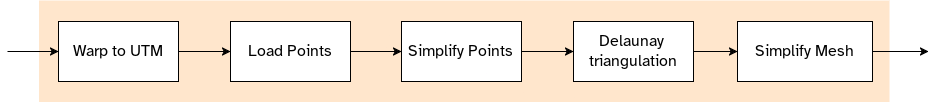
\includegraphics[width=1\textwidth]{assets/meshConstruction_zoomed.png}
  \caption{Flow graph showing the process required to generate a mesh from DEM data}\label{fig:mesh_construction:dataprocessing}
\end{figure}

\autoref{fig:mesh_construction:dataprocessing} outlines the pipeline from initial WGS84 DEM dataset to Delaunay Triangulation. The choice to simplify the point-set before triangulation, and again simplify the mesh after simplification was designed to allow for an exploration into performance differences and tweaks to the simplification, which are discussed later (see \autoref{section:impl:simplification}.).

\subsubsection{Data Feature Representation}

% % TODO: MOVE TO WHEN FEATURE CONTOURS ARE DISCUSSED
% After considering the potential features that may be useful in routing decisions, only the height of elevation was considered important. Whilst the x,y positions of features such as fences, buildings, and water are important, their height is not important. This means that the construction of the topography of the mesh is solely dependent on the DEM elevation data. The potential for future research into potential uses for enabling features to change z-coordinates of mesh points is discussed in \autoref{section:improvements:heightdata}.

Due to the limitations of W. Evans' approach of constructing the search graph solely using topography data, this project developed a novel approach to more accurately represent feature data within the search graph.

Two types of features were identified: area features, and edge features. When traversing over an edge, some features relate more to the surface (i.e. terrain area) being traversed; whereas others relate to the path itself (i.e. edge). For example, terrain type is best categorized as an area feature, as it's volume over the surface is meaningful. Paths, however, are often best represented as edge features, as their width is often is irrelevant to travel on-foot.

The approach to representing these features accurately is similar but requires slightly different setup. Overal, the process aims to apply the geoemtry of both types of features as constraints in the delaunay triangulation.

For edge features, adding a constraint onto the mesh ensures that edge exists in the final mesh. For area features, we can ensure that feature tagging can be done accurately by applying the edges of data into the mesh as constraints. This ensures that the border of data are maintained with edges, allowing traversal avoiding that particular feature, and ensures no faces overlap the border, preventing issues where a face could be tagged with either data value depeneding on where in the face is used for tagging.

These constraints are added based on the $X,Y$ coordinates of the contours, and are placed at the relevant $Z$ coordinate on the original mesh to prevent unwanted changes to the topography.

This method works well for most features, as mapping data usually impact the whole area specified, and does not come with height data. Therefore, this approach is likely sufficient to model most useful data features (i.e. paths, terrain types, building positions, etc.). Some notable 3D features that cannot be represented however are: heights of bridges, which may be relevant due to the fear-of-height response; and the height of objects which may be climbable (although legal restrictions usually prevent climbing over objects captured in GIS datasets).

\subsubsection{Vector Features}

As mentioned, representing area and edge features requires fetching edges and contours of data.

\subsubsection{Raster Features}

As mentioned, representing area features requires fetching

\begin{figure}[!htbp]
  \centering
  \subfloat[CEH Terrain Data]{
    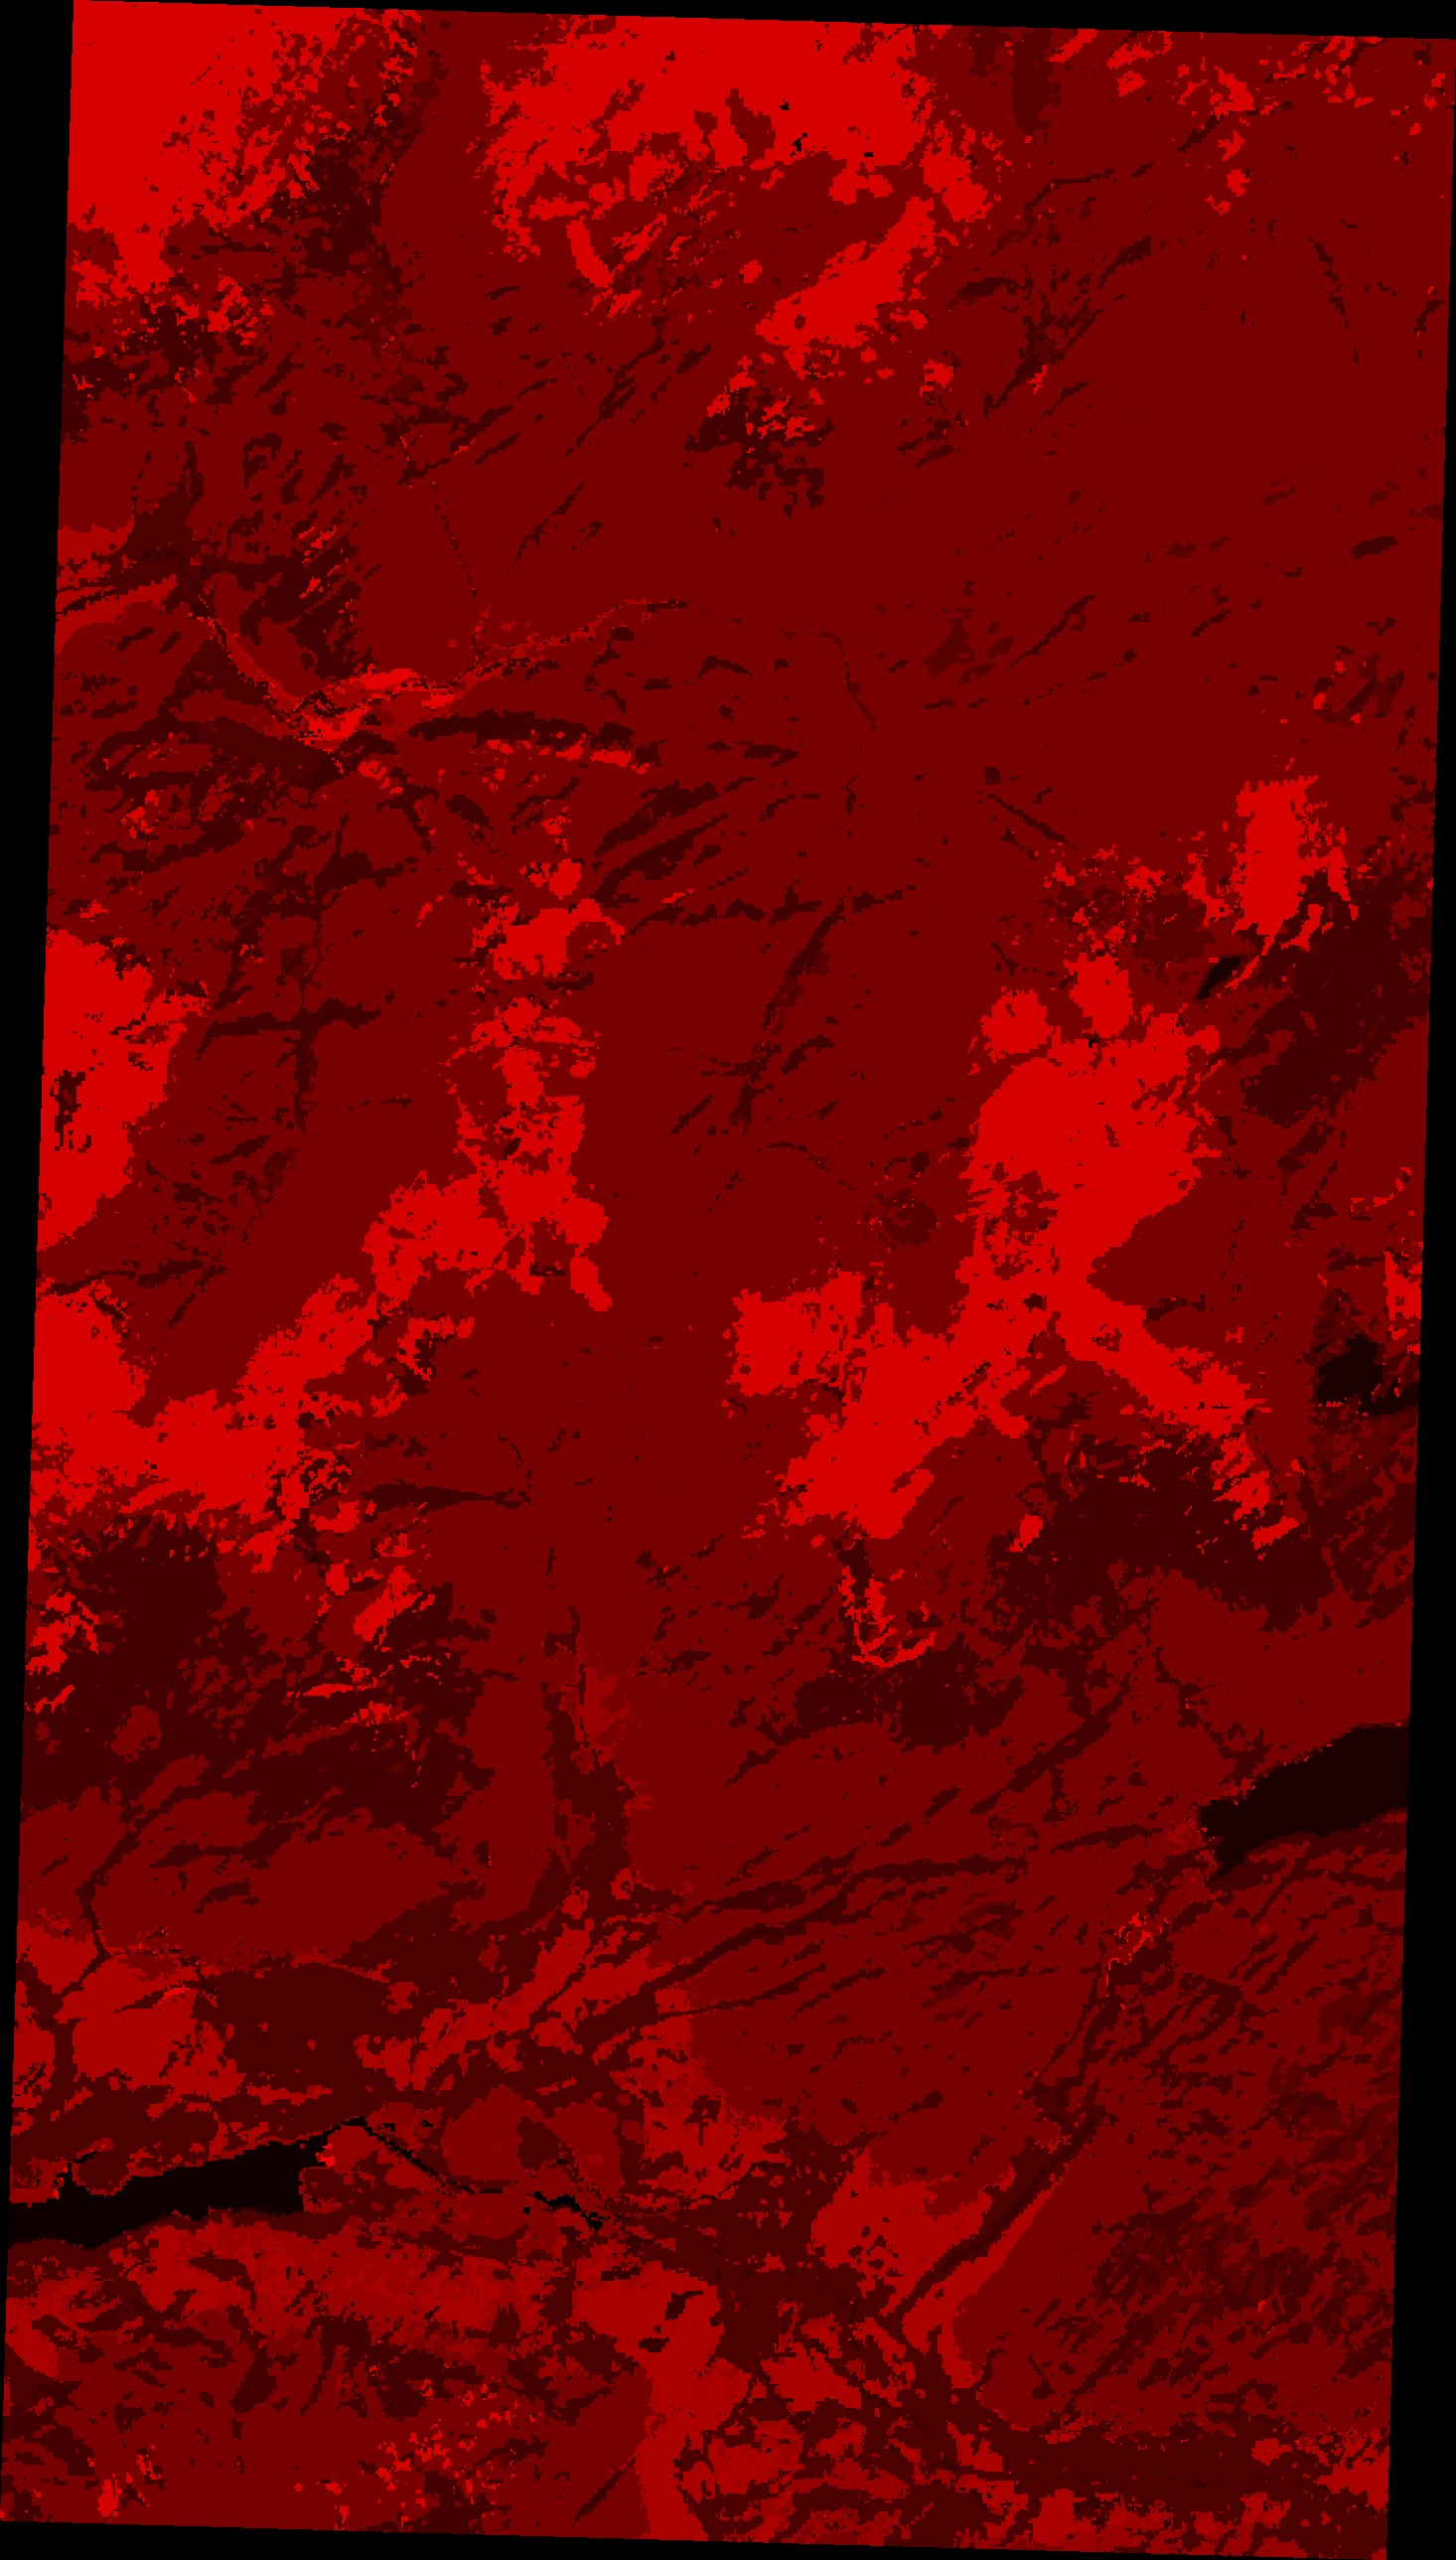
\includegraphics[width=0.35\textwidth]{assets/benNevis_chunk_terrain.png}
  }
  \subfloat[Detected Edges of the CEH Terrain Data] {
    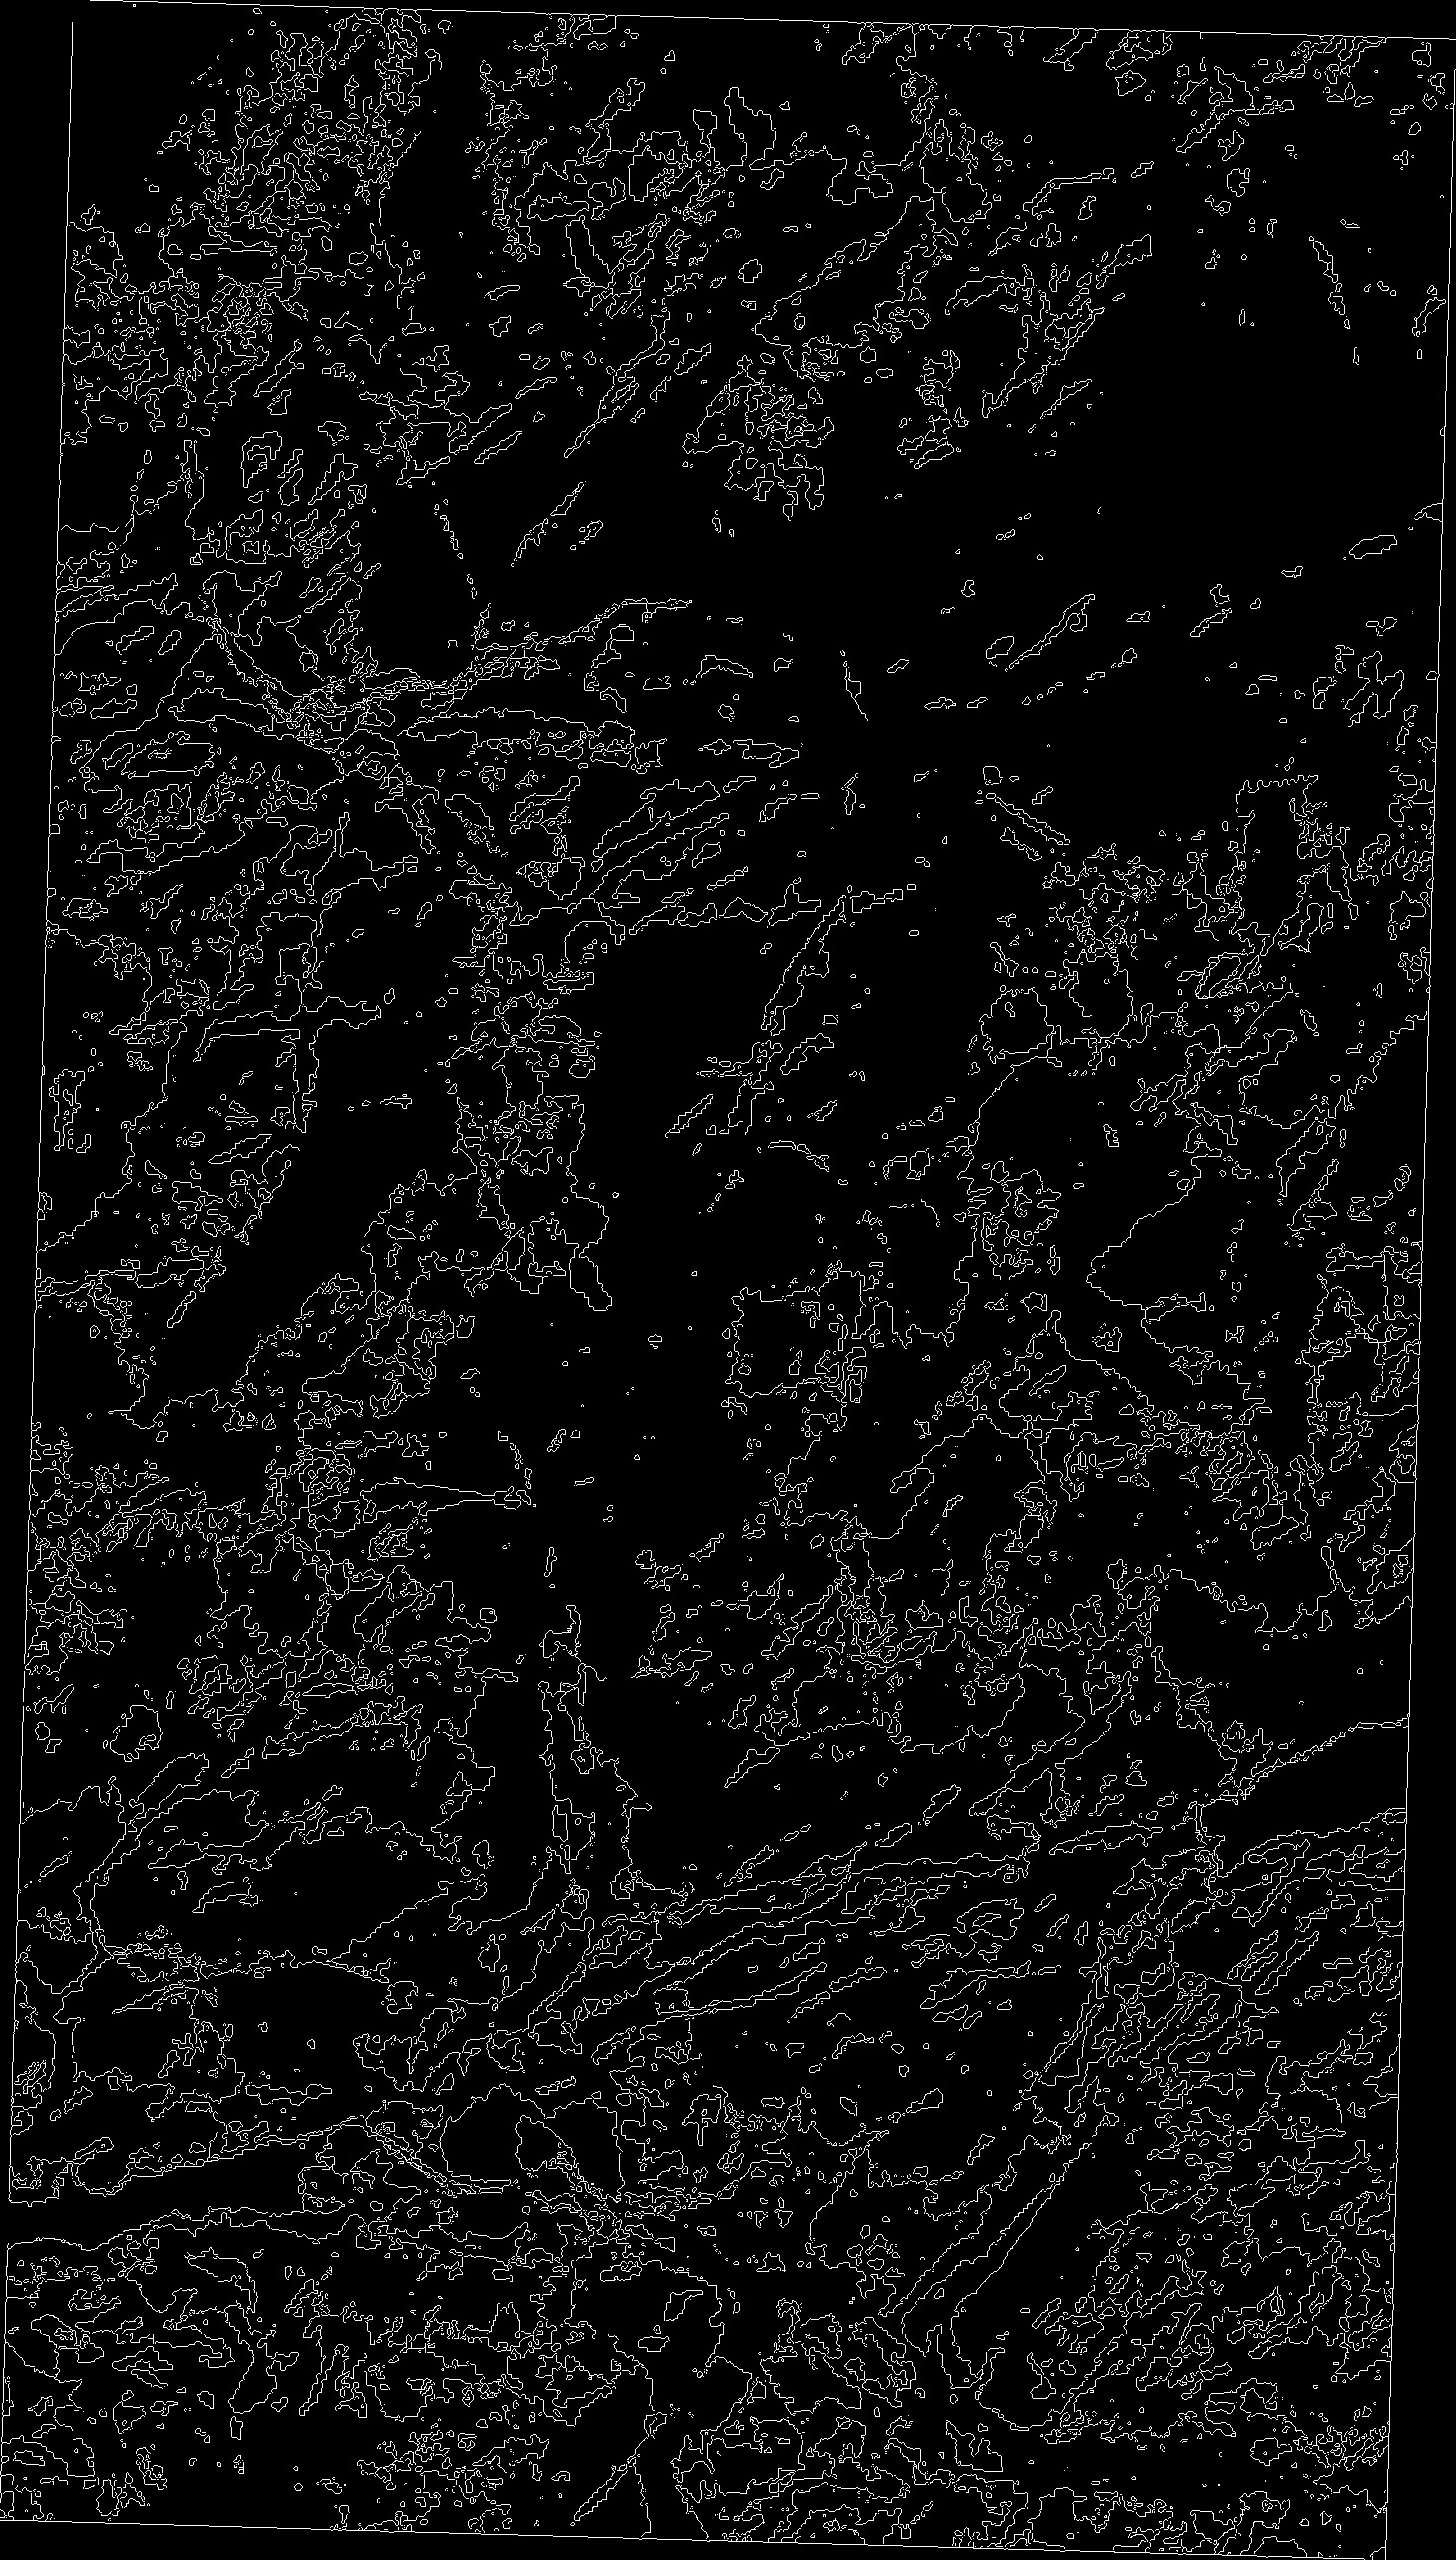
\includegraphics[width=0.35\textwidth]{assets/benNevis_chunk_edges.png}
  }
  \caption{The edges detected from a chunk of terrain-type data warped to UTM.}\label{fig:edges:terrain}
\end{figure}

% TODO: Context survey computer vision
Computer vision enables vector edges to be detected and extracted from raster data, which can then be converted into a set of constraints that can be applied onto the mesh.

Applying data edges as constraints is sufficient to accurately represent feature locations.\ \autoref{fig:data:terrain} shows the detected contours overlaid onto the original terrain type data. Every region defined by the contours have a uniform terrain type. Constraints ensure that edges fully cover each data border, and so every triangle will fall within, and not overlap any, terrain section --- getting the pixel value for any point in these triangles will therefore give the correct terrain type.

Using constraints to define data borders enables a high accuracy dataset to be represented even on a low DEM resolution mesh.

\subsubsection{Edge Features}

As discussed in \autoref{section:context:er:graph}, constructing the search graph solely based on geometry fails to accurately represent topological features with a higher resolution than the underlying DEM data. For simplified meshes, this issue is amplified as a highly-simplified mesh will have even fewer resolution for feature data.

\subsection{Routing Algorithm}

The design of the routing algorithm itself uses uniform cost search, with a custom modular cost function. Whilst A* would be more performant in many cases where there is an admissible heuristic, the admissibility of a heuristic is tied to the cost function, which here is designed to change and be customized with new features are relationships. Therefore, an admissible heuristic for one particular cost function would not be admissible for another. The ability to add heuristics could be relatively simply added, but given the wide target audience would need to be designed to protect against inadmissible heuristics.

\subsubsection{Cost Function}
% TODO: Discuss the design of the features themselves

\begin{figure}[!htbp]
  \centering
  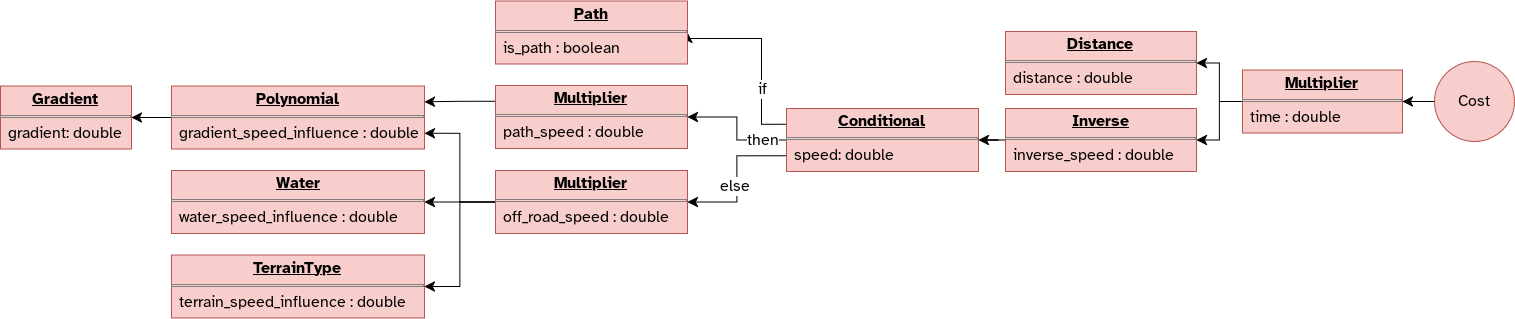
\includegraphics[width=\textwidth]{assets/costfunction_example1.png}
  \caption{Example DAG cost function design. Output models an estimated travel time using three factors influencing travel speed.}\label{fig:cost:example:1}
\end{figure}

A primary contribution this project has made is with the design of the cost function. The cost function is represented as a directed acyclic graph (DAG) of features, where each feature outputs a single value per cost-calculation, and connections between features allows the output of one feature to be used as an input to another feature forming dependencies.


\autoref{fig:cost:example:1} demonstrates the capacity for the cost function to model mathematical functions. Here, the model estimates travel time following the calculation:

\[\text{Time} = \frac{\text{Distance}}{\text{Speed}} = \text{Distance} \times \frac{1}{\text{Speed}}\]

\subsubsection{Features}

Features are designed to be able to represent any data or mathematical concept. Each feature follows the same three step setup process.

\begin{figure}[!htbp]
  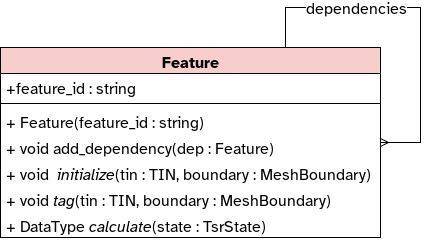
\includegraphics[width=0.5\textwidth]{assets/feature.png}
  \centering
  \caption{Feature class UMl design.}\label{fig:feature}
\end{figure}

First, a feature instance is created using the constructor. This default constructor can be overridden to enable additional configuration options to be set. Next, the function is initialized --- this is designed to enable features to fetch data from APIs if require, and modify the search graph as required. Finally, tagging enables features to setup data structures with the final search mesh.

Feature are designed to be able to override the default constructor. The default just sets the feature ID.\@ Here, other configuration options can be set with new parameters, as the function template for the \texttt{initialize} and \texttt{tag} functions should not be altered to enable these functions to be called automatically upon setup.

As shown in \autoref{fig:feature}, the initialize and tag methods are abstract, meaning each feature must define their own methods following this template. This allows features to implement empty methods if no configuration is required, such as a purely mathematical feature such as the gradient or distance features, or call APIs and cache results such as with the \texttt{PathFeature}, \texttt{WaterFeature}, and \texttt{CEHTerrainFeature}.

The calculation logic must also be defined by each feature. Features are designed to be able to output any type of information, as some data types are categorical, some quantifiable, etc. When using dependencies, the dependent will call the dependency function's calculate function, and this output type must match the expected type. The final output feature must be a number representing the non-negative cost.

\subsubsection{Data Features}

Whilst all feature types are treated the same, it is useful to distinguish data features, with logic features. Logic features take input, apply some logic, and output the value. Data features use datasets to give information about some feature of the terrain.

Every data feature will require a very similar design to their initialization and tagging setup functions.

\subsection{Graph Traversal}

Dijkstra's algorithm was selected to serve as the basis of this search algorithm. Specifically, uniform cost search, as the ultimate goal is to find the optimal route between two nodes. Uniform cost has lower space complexity due to the storage of a best-cost only once the node has been searched, unlike Dijkstra's initial design which requires setting all nodes to infinity best-cost initially.

\subsection{API}

Constructing both the initial topographical TIN and setting up data features require datasets from online APIs. Given a search, this application is designed to automatically fetch the GIS data required. These APIs have different, yet similar formats, and designing a simple interface that can be customized to work for any API format makes adding new features easier. Having automatic fetching of data from APIs is important for the user-experience and accessibility of the application, as otherwise each dataset would have to be manually downloaded and given to the application in some way.

\subsection{Chunking}

\begin{figure}[!htbp]
  \centering
  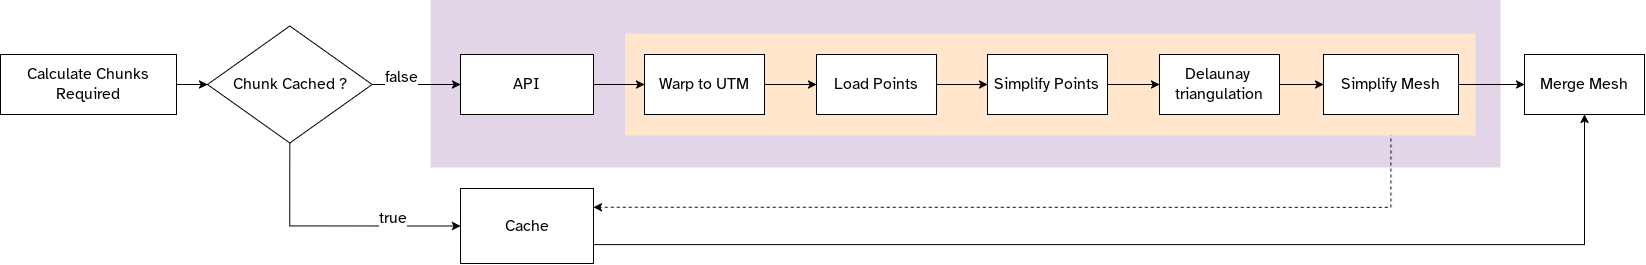
\includegraphics[width=1\textwidth]{assets/meshConstruction.png}
  \caption{Final search graph construction process with automatic chunking, api calling, and caching.}\label{fig:mesh_construction:full}
\end{figure}

For extensive searches, the system efficiently handles large volumes of Digital Elevation Model (DEM) and feature data by dividing it into manageable square tiles of a specified size. This method, known as chunking, ensures that data is loaded and processed safely while maintaining consistent partitioning across different uses of the application.

By automatically dividing land into uniform tiles, the system optimizes API calls and caching. This reduces the number of requests and processing required for subsequent searches, improving both speed and efficiency. Entire tiles are downloaded and processed, including those overlapping the search boundary, allowing complete caching of these tiles for future use.

This approach minimizes redundant data retrieval, accelerates operations, and ensures seamless handling of large datasets. It not only enhances performance but also reduces computational and network resource demands, making the system robust and scalable.

\subsubsection{Parallelism}

\begin{figure}[!htbp]
  \centering
  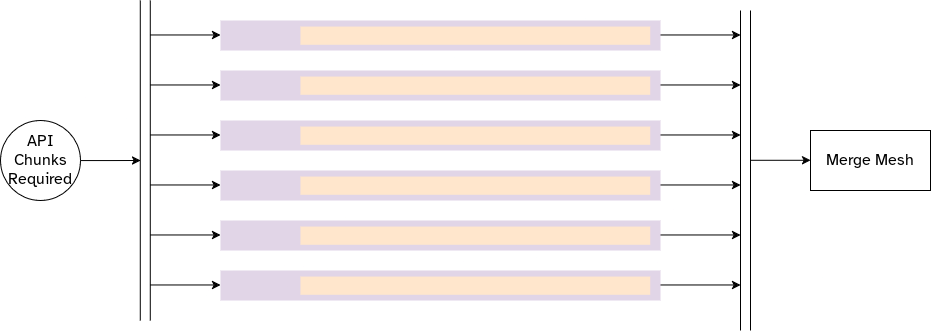
\includegraphics[width=1\textwidth]{assets/meshConstruction_parallel.png}
  \caption{Parallel design of processing DEM chunks into a completed TIN.}
\end{figure}

After the required chunks are determined, the process of fetching the data from the API and constructing the mesh shown in \autoref{fig:mesh_construction:thread} is designed to be completely independent for each chunk, and only once all chunks are processed are merged together. This enables a pipeline parallelism structure to be designed.

\subsubsection{Caching}

Caching data is used to dramatically reduce the API calls and processing requirements required for subsequent searches with overlapping search boundaries.


% TODO: Implementation section
\section{Implementation}

An important note for this section: some UML diagrams display pointers with asterisks (e.g.\ \texttt{Feature *}). Please note that unless otherwise stated, these are all referring to smart pointers in their implementation, as manual malloc/free pointer creation requires manual memory management. Smart pointers are favoured to automatically free out-of-scope variables, preventing memory leaks.

% TODO: mesh derivation (CGAL), features (inheritance and overriding functions, dependencies local to features, OpenCV computer vision), data files (warping, GDAL), API (libcurl), optimization (multi-threading/oneTBB), caching (database vs local files), visualization (KML)

% TODO: mesh derivation, 

\subsection{Mesh Derivation}

CGAL was used for converting the DEMs to TINs. CGAL offers constrained Delaunay trinagulation, which is an essential design feature of the mesh. In addition, to enable initial experimentation with mesh optimisation, CGAL does not impose a limit to the number of components in the mesh like the Fade library.

CGAL's constrained Delaunay triangulation is done automatically by the \texttt{Constrained_\allowbreak{}Delauany_\allowbreak{}Triangulation_2} class. CGAL enables 2.5D triangulation through this class, with the addition of the \texttt{Projection_\allowbreak{}Traits_\allowbreak{}_xy_3}. This triangulates points on the $xy$ plane, and then applies the $z$ position onto those points.

This 2D Delaunay triangulation projected onto 3D is less complex than using a 3D Delaunay triangulation, which constructs tetrahedra. \textcite{perkins2013fielddstar} found that routing over tetrahedra is also less performant. In addition, the DEM data used is 2.5D, and so little benefit would be gained from a 3D triangulation.

\subsection{Features}

\begin{figure}[!htbp]
  \centering
  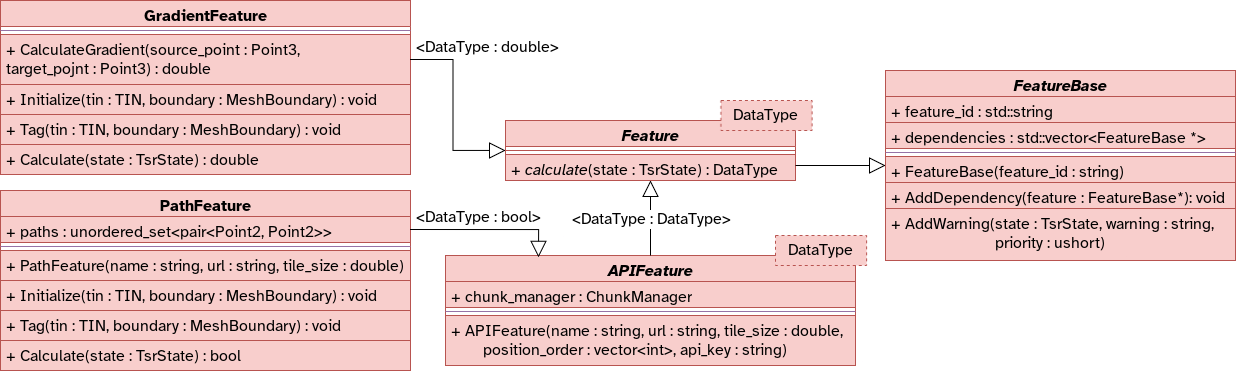
\includegraphics[width=\textwidth]{assets/FeatureBase.png}
  \caption{UML diagram showing the basic FeatureBase and Feature interfaces, with the specialized APIFeature interface, and two example of actual Features that can be instantiated.}\label{impl:features:uml}
\end{figure}

% TODO: Discuss the generic feature interface
% TODO: Discuss each individual feature
% TODO: Discuss the 

\subsection{Raster Feature Edge Detection}

As mentioned in the design section, raster area features use computer vision to detect the edges and convert them to vector contours. The edge detection itself is handled by the OpenCV library, offering canny edge detection, which detects sharp changes in values (i.e. data borders).

The \texttt{CEHTerrainFeature} and \texttt{WaterFeature} show example usage of this technique. First, the


use the OpenCV computer vision library to detect edges in their raster datasets, and convert them to a vector of vectors representing individual edges to apply as contours.

\subsection{Raster Position Extraction}

Relating pixel values to the position


\subsection{Coordinate System Conversion}

Warping raster datasets requires a different approach than warping vector datasets. For raster data, GDAL's \texttt{GDALWarp} tool was used, which handles resampling and re-projection of datasets. For vector datasets, \texttt{GDALTranslate} was used to warp the vector points and geometries. These tools ensure efficient and accurate coordinate system conversions.

The decision to use GDAL instead of developing custom warping tools was driven by GDAL's proven optimization for performance and memory management. These factors are critical for the efficiency of the routing algorithm, as computational overhead can significantly impact results. GDAL's C++ APIs are well-documented and support a wide range of input file types and projections, streamlining the implementation process.

% TODO: Results section
\section{Results and Analysis}

This section explores how different configurations and inputs affect the performance of the router in terms of both performance and quality of routes. Visualization of the generated meshes themselves is done through exporting the mesh to an object file, which is imported into the popular 3D modelling tool blender.

\subsection{Final Configuration Mesh Generation}

Objectively determining the quality of the mesh triangulation is not possible, as there are an infinite number of triangulations that could represent the same terrain. However, we can identify features in meshes which may give insights into their quality.

\begin{figure}[!htbp]
  \subfloat[TSR's Solid Mesh] {
    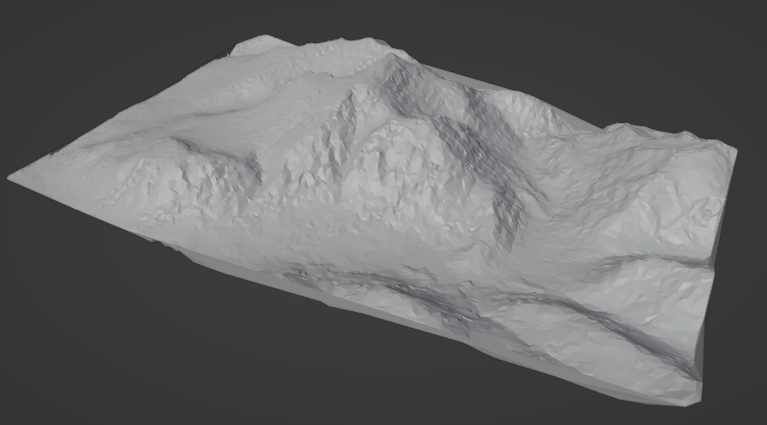
\includegraphics[width=0.4\textwidth]{assets/benNevis_perspective_solid.png}
  }
  \subfloat[Google Earth's Topography] {
    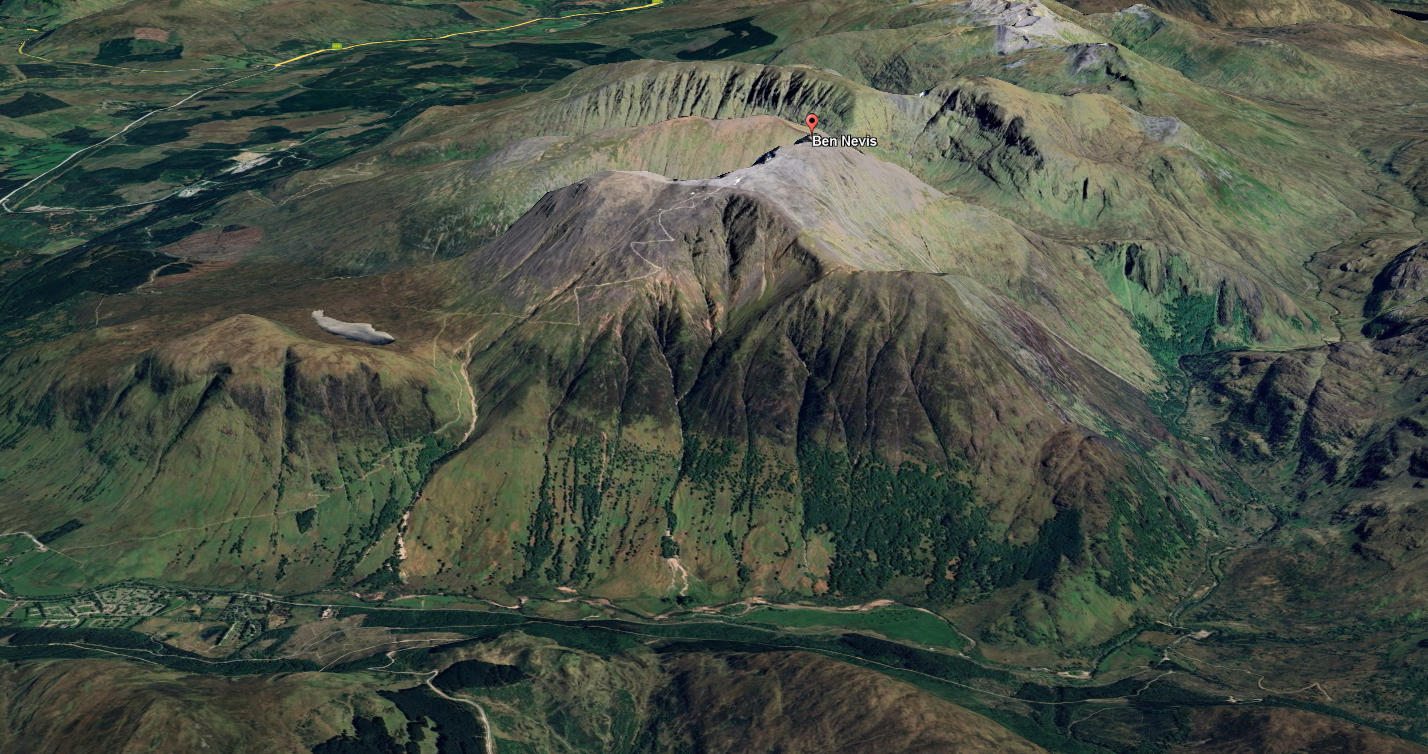
\includegraphics[width=0.4\textwidth]{assets/benNevis_gearth.png}
  }
  \caption{Visual comparison of meshes of Ben Nevis. The generated mesh from this application on the left, and Google Earth's topology mesh on the right.}\label{fig:mesh:ben_nevis:comparison}
\end{figure}

We initially evaluate the accuracy of the generated TIN mesh by visually comparing it to Google Earth's topography, as shown in \autoref{fig:mesh:ben_nevis:comparison}. Google Earth's horizontal accuracy (~30m) and height accuracy (~10m), are only marginally higher than the COP-30 DEM used in this project. Therefore, significant differences between the two meshes are likely a result of the mesh simplification process.

However, one limitation of this comparison arises from the differing projections used. Google Earth uses the WGS84 projection scheme, not UTM, and so there are some scaling and warping due to this difference. However, general features should still be identifiable.

As seen in \autoref{fig:mesh:ben_nevis:comparison}, the primary topographic features in the Google Earth mesh are all visible in the generated mesh. Nonetheless, improvements could be made in finer details such as sharp angles in mountain ridges, and sudden valleys.

In addition, the DEM data used fails to accurately model the topography of areas under water, as seen in the bottom left of \autoref{fig:mesh:ben_nevis:comparison}. However, this does not impact the quality of most routes as usually water is completely avoided, or otherwise the water is swam through, at the surface.

\subsubsection{Edge Detection}

\begin{figure}[!htbp]
  \centering
  \subfloat{
    \centering
    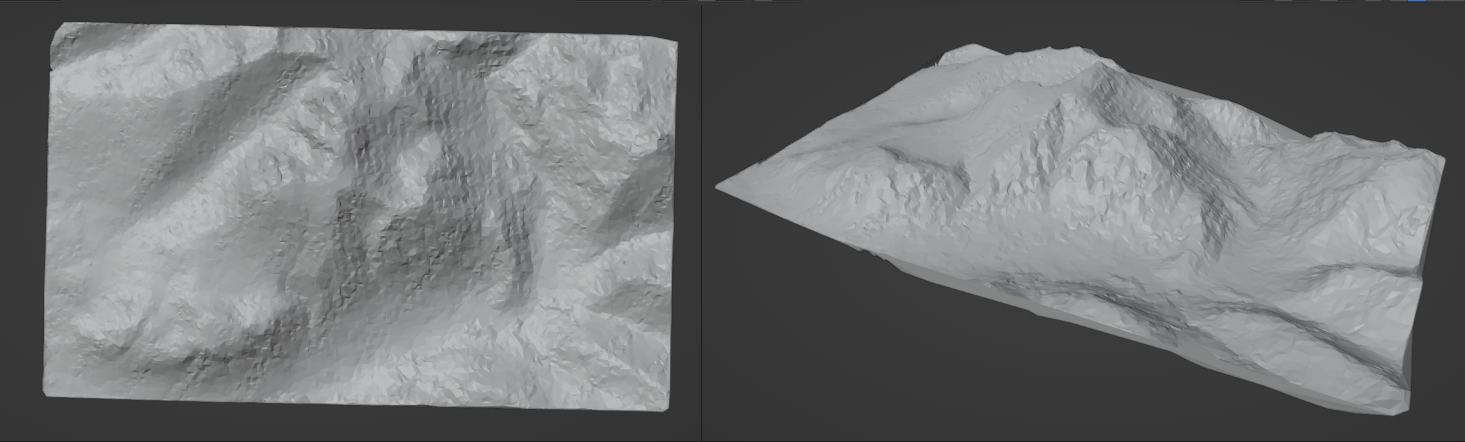
\includegraphics[width=0.8\textwidth]{assets/benNevis.png}\label{fig:mesh:ben_nevis:solid}
  }\\
  \subfloat{
    \centering
    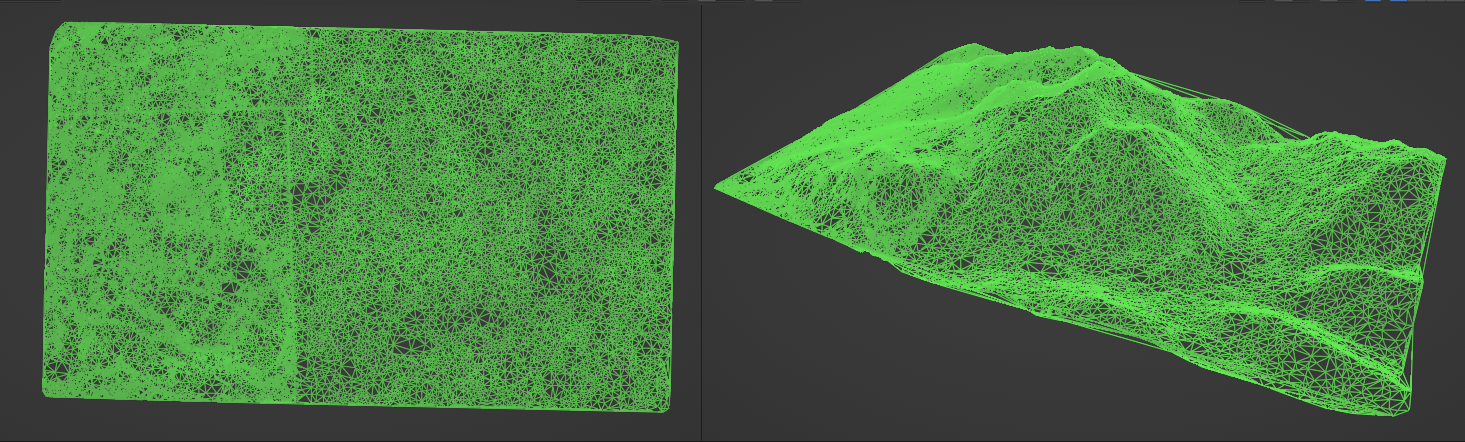
\includegraphics[width=0.8\textwidth]{assets/benNevis_wire.png}\label{fig:mesh:ben_nevis:wireframe}
  }
  \caption{Final model of Ben Nevis, with path, water-feature, and terrain-type contours applied. A solid and wireframe render are shown, in both top-down orthographic, and side-on perspective views. Demonstrating a recognizable, but noisy and non-perfectly optimized mesh.}\label{fig:mesh:ben_nevis}
\end{figure}

\autoref{fig:edges:terrain} and \autoref{fig:mesh:ben_nevis} demonstrate a drawback to the edge-detection implementation. For each chunk, a different image is used which is warped before fetching the contours. This means that the images have areas of NO\_DATA values, and the border between NO\_DATA and any value is detected as an edge. An alternative approach could be to run the edge-detection before warping, and using a vector warping on the resulting edges. It would be easier here to prevent edges on the border of images being included as contours in the final mesh.

\subsection{Generated Routes}

This section analyzes the routes generated by this route planner, considering differences between different cost function pre-sets. Evaluation therefore will be focused on the success to which the cost function generates routes according to the goal of the model.

The first preset can be found in \autoref{fig:cost:example:1} and models estimated traversal time. Three features are considered

\subsection{Performance}

The route planner has multiple major factors influencing the performance of any particular execution which will be discussed and analyzed here.

Performance is analyzed in two parts: search graph construction, and then the actual routing. This enables a focused comparison of performance for different cost function models.

\subsubsection{Mesh Size}

\subsubsection{Cost Function Complexity}

\subsubsection{Caching}

% TODO: Evaluation section
\section{Evaluation and Critical Appraisal}

% TODO: Potential Improvement & Future Projects
\section{Potential Improvements \& Future Projects}

This project aimed at forwarding research into accessible off-road route planning. Due to the scale of route planning off-road, and the limited previous research, this solution to the problem is not perfect. This section discusses these potential improvements in detail, along with a discussion of some of the extraneous research that would need to be done to solve some of the limitations of this project.

\subsection{Parallel Route Search}

% TODO: threading search
% TODO: threading feature initialization / pre-processing
% TODO: use a database for caching datasets
% TODO: errors around the sides of meshes
% TODO: further mesh optimizations / processing
% TODO: caching of results when features used in multiple parts of cost function
% TODO: analysis of tile size for API / cache calls - potentially separate API call tile size and cache tile size

\subsection{Modelling Features}

All of the data features constructed for this application were fundamentally first-attempts at quantification of some of the key features impacting routing preference.

This section outlines some improvements that could be made to the existing features, and possible additional features that would increase the modelling capacity of the route planner.

\subsubsection{Distance Dependent Features}

The implementation of the water feature created allows avoiding or heavily punishing swimming. However, it may be helpful to set a maximum swimming distance, to ensure routes through overly large areas of water are suggested.

This could be done by first getting the distance for the current edge if it is over water. If beyond a determined maximum swimming length, then it could return an infinite cost (implying non-traversable). If lower, then the source vertex's parent could be fetched from the \texttt{bestRoutes} map in the state. We can repeatedly check if that edge is over water, and add the distance to a running total until you reach land, to get the total current water distance.

Alternatively, a more performant approach may be to change the RouteNode class, and make it possible for Calculate methods to cache their calculated values to each Node, which could include a cumulative water distance, allowing future nodes to fetch this value instead of calculating for every cost-evaluation.

\subsubsection{Cost Function Caching}

Whilst there is pre-caching of many data-values, additional caching at-runtime for a particular cost-function evaluation may dramatically improve performance for more complex models.

The DAG structure enables multiple nodes to add dependencies to the same node as long as there are no cycles. However, each of these nodes calls the Calculate function separately.

One solution to this problem may be to cache values when a method is called first, and so subsequent calls do not require redundant calculation.

\subsection{Iterative Cost Function}

Due to new stack frames being generated at each function call, the current recursive design of the cost function limits it's maximum size and complexity, as each dependency runs whilst the parents function is still in scope, thus using memory. Performance in all aspects could be improved through the conversion of this recursive design to an iterative approach.

This may involve using the FeatureManager to handle all calculate requests. Instead of features directly calling calculate to their dependencies and casting these results, the feature manager could maintain a list of the dependencies, and iteratively follow the DAG, not calling calculate until a leaf-node is found (one with no dependencies). The leaf nodes could then be calculated and their values passed as input when calling calculate on it's dependent.

However, challenges arise in maintaining the ability for features to output any type, as the feature manager would have to be able to handle the arbitrary output type, and input it into features.

\section{Conclusion}

\pagebreak

\nocite{esa2024dem}
\nocite{cgal:eb-24b}
\nocite{rouault_2022_6517191}
\nocite{wiki:osm}
\nocite{gtest}
\nocite{fmtlib}
\nocite{opencv_library}
\nocite{oneTBB}
\nocite{tin_terrain_logging}
\nocite{libboost}
\nocite{geographiclib}

\printbibliography[heading=bibnumbered]{}

\pagebreak
\begin{appendices}

  \section{System Requirements}

  The following is a list of required c++ libraries that need to be installed. The version used in testing is also given.

  \begin{itemize}
    \item GDAL
    \item CGAL
    \item oneTBB
    \item openCV
    \item GeographicLib
    \item
  \end{itemize}

  \section{Compilation Instructions}

  To build the library and router, first setup the build directory:

  \begin{lstlisting}[language=bash]
  \$ cd tsr-cli
  \$ mkdir build && cd build
\end{lstlisting}

  \noindent Then configure with \texttt{cmake}, making sure to set configuration option values as appropriate:

  \begin{lstlisting}[language=bash]
  \$ cmake .. -G Ninja -DCMAKE_BUILD_TYPE= -DTSR_TEST=
\end{lstlisting}

  \vspace*{-2em}

  \begin{itemize}
    \item \texttt{TSR\_TEST=ON/OFF}

          Specify whether to build test suite.

    \item \texttt{CMAKE\_BUILD\_TYPE=Release/Debug}

          Specify build type. Release is far more performant, but Debug contains much more logging information.
  \end{itemize}


  \noindent The library, cli-app, and tests can then be compiled using one of the following:

  \begin{lstlisting}[language=bash]
  # Compile everything
  \$ ninja

  # Compile just the library
  \$ ninja tsr

  # Compile the tests
  \$ ninja test-tsr

  # Compile the cli application
  \$ ninja tsr-cli
\end{lstlisting}

  \pagebreak
  \section{User Manual}

  For the cli applicaiton, refer to the user manual below:

  \begin{lstlisting}[]
  Usage: 
      tsr-cli [options] <start_lat> <start_lng> <end_lat> <end_lng>
        Route between the given start and end points
      tsr-cli [options] --example  
        Route between a set of example start and end points

    Options:
      --radii-multiplier  Radii multiplier to apply to domain size
      --output-dir        Directory to put output files
      --cache-dir         Tile cache directory
      --quiet             Reduce stdout output
\end{lstlisting}

  For the web application, run the development server with the following:

  \begin{lstlisting}[language=bash]
  \$ cd tsr-ui
  \$ npm run dev
\end{lstlisting}

  \pagebreak
  
\includepdf[pages=1, scale=0.8, pagecommand=\section{Ethics Self-Assessment Form}\label{appendix:ethics}]{ethics.pdf}
  
\includepdf[pages=2-, scale=0.8]{ethics.pdf}

\end{appendices}

\end{document}